\documentclass{report}
\usepackage[T1]{fontenc} % Fontes T1
\usepackage[utf8]{inputenc} % Input UTF8
%\usepackage[backend=biber, style=ieee]{biblatex} % para usar bibliografia
%\usepackage{csquotes}
\usepackage[portuguese]{babel}
%\usepackage[portuguese]{babel} %Usar língua portuguesa
\usepackage{blindtext} % Gerar texto automaticamente
\usepackage[printonlyused]{acronym}
\usepackage{hyperref} % para autoref
%\usepackage{graphicx}
\usepackage[pdftex]{color,graphicx}

\usepackage{amsmath}

% Pacote para a definição de novas cores
\usepackage{xcolor}
% Definindo novas cores
\definecolor{verde}{rgb}{0.25,0.5,0.35}
\definecolor{jpurple}{rgb}{0.5,0,0.35}
\definecolor{darkgreen}{rgb}{0.0, 0.2, 0.13}
%\definecolor{oldmauve}{rgb}{0.4, 0.19, 0.28}
% Configurando layout para mostrar codigos Java
\usepackage{listings}

\newcommand{\estiloC}{
\lstset{
    language=C++,
    basicstyle=\ttfamily\small,
    keywordstyle=\color{jpurple}\bfseries,
    stringstyle=\color{red},
    commentstyle=\color{verde},
    morecomment=[s][\color{blue}]{/**}{*/},
    extendedchars=true,
    showspaces=false,
    showstringspaces=false,
    numbers=left,
    numberstyle=\tiny,
    breaklines=true,
    backgroundcolor=\color{cyan!10},
    breakautoindent=true,
    captionpos=b,
    xleftmargin=0pt,
    tabsize=2
}}


\bibliography{bibliografia}


\begin{document}
%%
% Definições
%
\def\titulo{Informação e Codificação}
\def\subtitle{Projeto 2}
\def\data{04 de dezembro de 2022}
\def\autores{Bruno Silva (97931)brunosilva16@ua.pt \\ Marta Oliveira (97613) marta.alex@ua.pt \\ Mariana Silva (98392) marianabarbara@ua.pt}
\def\versao{VERSAO 1}
\def\departamento{DETI}
\def\empresa{Universidade de Aveiro}
\def\logotipo{ua.pdf}
%
%%%%%% CAPA %%%%%%
%
\renewcommand{\contentsname}{Índice}
\begin{titlepage}

\begin{center}
%
\vspace*{15mm}
%
{\Huge \titulo}\\
%
\vspace{10mm}
%
{\Huge \subtitle}\\
%
\vspace{10mm}
%
{\Large \empresa}\\
%
\vspace{10mm}
%
{\LARGE \autores}\\ 
%
\vspace{10mm}
%
\begin{figure}[h]
\center
\includegraphics{\logotipo}
\end{figure}
%
\vspace{30mm}
\end{center}
%
\begin{flushright}
\versao
\end{flushright}
\end{titlepage}

%%  Página de Título %%
\title{%
{\Huge\textbf{\titulo}}\\
{\Large \departamento\\ \empresa}
}
%
\author{%
    \autores
}
%
\date{\data}
%
\maketitle

\pagenumbering{roman}



%%%%%% Agradecimentos %%%%%%
% Segundo glisc deveria aparecer após conclusão...
%\renewcommand{\abstractname}{Agradecimentos}
%\begin{abstract}
%Eventuais agradecimentos.
%Comentar bloco caso não existam agradecimentos a fazer.
%\end{abstract}


\tableofcontents
 %\listoftables     % descomentar se necessário
 %\listoffigures    % descomentar se necessário


%%%%%%%%%%%%%%%%%%%%%%%%%%%%%%%
\clearpage
\pagenumbering{arabic}

%%%%%%%%%%%%%%%%%%%%%%%%%%%%%%%%
\chapter{Introdução}
\label{chap.introducao}
\paragraph{}
O presente relatório tem como objetivo descrever a resolução do Projeto 2 desenvolvido no âmbito da unidade curricular de Informação e Codificação.
\paragraph{}
O código desenvolvido para o projeto encontra-se disponível em \url{https://github.com/brunosilva16/IC/tree/main/proj2}
\paragraph{}
Para este projeto utilizamos a biblioteca \textit{openCV}.
\paragraph{}
No ficheiro README.md no repositório estão as indicações de como compilar cada exercício.


\chapter{Parte I}
\label{chap.ParteI}
\section{Exercício 1}
\paragraph{}
No exercício 1 era pedido que se implementasse um programa que fizesse a cópia de uma imagem, píxel por píxel, de um ficheiro para o outro. Para isso, necessitamos de um ficheiro de imagem (existente) para entrada e um nome de um ficheiro para ser criado como \textit{output}. Dessa forma, utilizámos da biblioteca \textit{OpenCV}.
\paragraph{}
Uma imagem é a representação de um conjunto de pontos definidos por valores numéricos, formando uma matriz onde cada ponto é um píxel.
\paragraph{}
Cada ponto de uma imagem é decomposto em uma tripla de cores, isto é, representam-se usando o modelo RGB(Red, Green, Blue).
\paragraph{}
Para conseguirmos representar as imagens criámos 2 objetos do tipo \textit{Mat}. Um representa a imagem original e outro vai representar a cópia (output).
\paragraph{}
Com o auxílio do tipo de dados \textit{Vec3b}, isto é, um vetor com 3 bytes de entrada onde cada byte vai representar a intensidade de cada canal de cor(vermelho, verde e azul), fornecendo um alcance de 256 possíveis valores, ou intensidades, para cada tom, conseguimos copiar píxel a píxel de uma imagem paraa outra. 
\paragraph{}
Com isto, realizámos o seguinte:
\begin{scriptsize}
\estiloC
\begin{lstlisting}[caption={Código fonte em C++}, label=lst:javacode]
	for(int i=0; i < image.rows; i++){
        for(int j=0 ; j < image.cols; j++)
            output.ptr<Vec3b>(i)[j] = Vec3b(image.ptr<Vec3b>(i)[j][0], image.ptr<Vec3b>(i)[j][1], image.ptr<Vec3b>(i)[j][2]);
    }
\end{lstlisting}
\end{scriptsize}
\paragraph{}
Através dos ciclos \textit{for} vão ser percorridos todos os píxeis da nossa imagem. 
\paragraph{}
De seguida, a informação obtida em cada uma das iterações dos ciclos é guardada num novo ficheiro de imagem.
\paragraph{}
\textbf{Como compilar:} make copy\textunderscore image
\paragraph{}
\textbf{Executar o programa:} ../opencv-example-bin/copy\textunderscore image <input\textunderscore file> <output\textunderscore file>

\section{Exercício 2}
\paragraph{}
Para este exercício implementámos um programa, igualmente utilizando a biblioteca \textit{OpenCV}, que produz vários efeitos.
\paragraph{}
	\begin{enumerate}
   	\item \textbf{Criar uma versão negativa de uma imagem.} \paragraph{}
   	   Para criar uma versão negativa de uma imagem temos que subtrair, a cada pixel que a constitui, o valor máximo de intensidade que é possível. Neste caso, este valor é 255, pois como explicámos no exercício anterior existe um alcance de 256 valores possíveis para cada tom.
   	   
   	   \paragraph{}
   	\begin{scriptsize}
    \estiloC
    \begin{lstlisting}[caption={Código fonte em C++ para criar o negativo da imagem}, label=lst:javacode]
    if(effect=="n"){
        Mat img2=255 - image; //Image negative is produced by subtracting each pixel from the maximum intensity value. e.g. for an 8-bit image, the max intensity value is 28– 1 = 255, 
        //thus each pixel is subtracted from 255 to produce the output image
        imshow("img2",img2); 
        waitKey(0);
        return 0; 
    } 
    \end{lstlisting}
    \end{scriptsize}

   	\paragraph{}
   	\paragraph{}
   	\textbf{Compilar programa:} make ex\textunderscore 2 \paragraph{}
   	\textbf{Executar programa:} ../opencv-example-bin/ex\textunderscore 2 <input\textunderscore file> n 
   	
   	\begin{figure}
    \centering
    \begin{minipage}{.5\textwidth}
    \centering
    
\includegraphics[width=0.8\linewidth]{teste.jpg}
    \captionof{Imagem Original}
    \label{fig:test}
    \end{minipage}%
    \begin{minipage}{.5\textwidth}
    \centering
    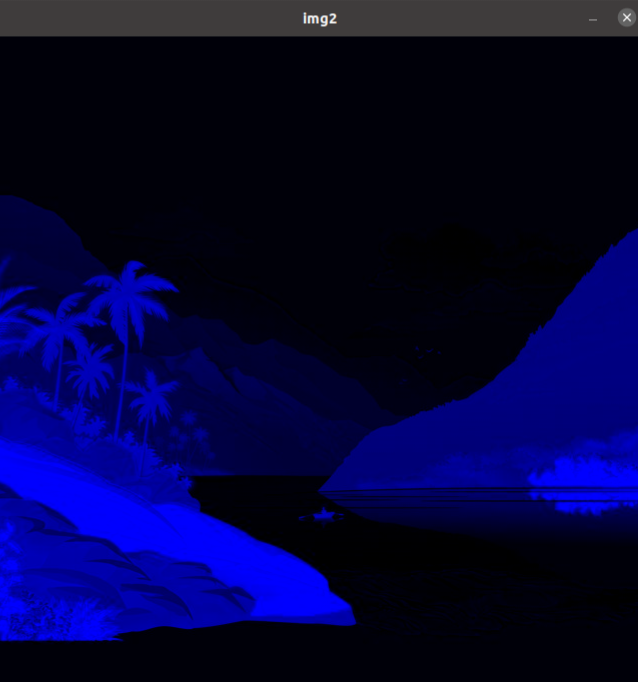
\includegraphics[width=.8\linewidth]{negative.png}
    \captionof{Negativo da Imagem}
    \label{fig:teste2}
    \end{minipage}
    \end{figure}
   	
   	\item \textbf{Criar uma versão espelhada de uma imagem (horizontalmente ou verticalmente).}
   	
   	\paragraph{}Para criar uma imagem espelhada, usufruimos de uma função própria do \textit{OpenCV}: \textit{flip}.
    \paragraph{}Esta função usa um \textit{flip code} para espelhar a imagem. Para espelhar no eixo do x coloca-se um '0' e no eixo dos y coloca-se um '1'.
    \paragraph{}
    Usando a mesma imagem para efeitos de testes , de seguida apresentamos os resultados da execução do código para ambos os tipos de espelhagem (horizontal e vertical).
    
   	\paragraph{}
   	\begin{scriptsize}
    \estiloC
   	\begin{lstlisting}[caption={Código fonte em C++ para espelhar a imagem}, label=lst:javacode]
   	if(effect=="m"){ //https://stackoverflow.com/questions/14907964/mirror-image-in-opencv
        Mat dst2;   
        cout<<"To flip image horizontally insert a '0' to flip vertically insert an '1'\n";
        int value;
        cout<<"choose value: "<<endl;
        cin>>value;
        //flip code: A flag to specify how to flip the array; 0 means flipping around the x-axis and positive value (for example, 1) means flipping around y-axis. 
        // //Negative value (for example, -1) means flipping around both axes. Return Value: It returns an image.
        if(value==0){
            Mat dst2;
            flip(image,dst2,0);
            imshow("flipped_horizontally",dst2);
            waitKey(0);
        }
        if(value==1){
            Mat dst2;
            flip(image,dst,1);
            imshow("flipped_vertically",dst);
            waitKey(0);
        }             
    }
    \end{lstlisting}
    \end{scriptsize}
    
    \begin{figure}[h!]
    \centering
    \begin{minipage}{.5\textwidth}
    \centering
    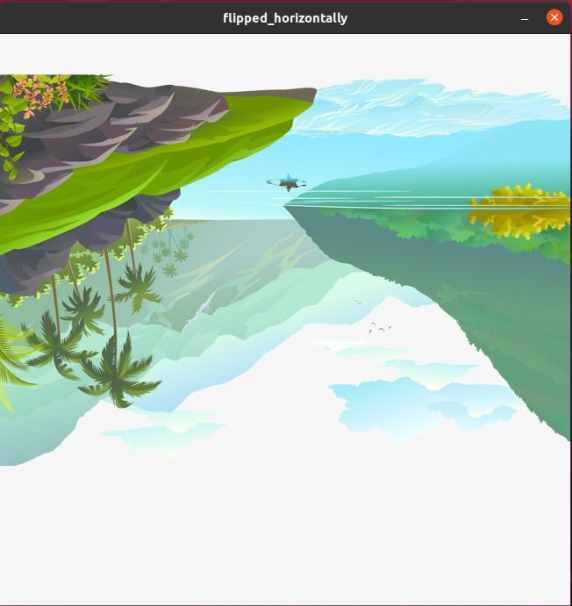
\includegraphics[width=0.8\linewidth]{flipped_horizontally.png}
    \captionof{Flipped Horizontally}
    \label{fig:flipped_horizontally}
    \end{minipage}%
    \begin{minipage}{.5\textwidth}
    \centering
    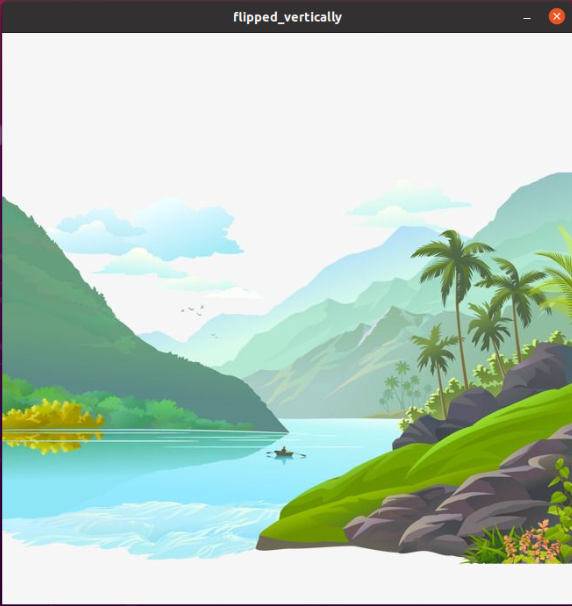
\includegraphics[width=.8\linewidth]{flipped_vertically.png}
    \captionof{Flipped Vertically}
    \label{fig:flipped_vertically}
    \end{minipage}
    \end{figure}
    
    \paragraph{}
    \begin{figure}[h!]
    \centering
    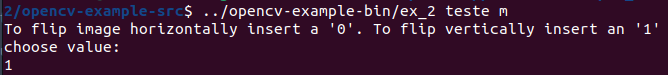
\includegraphics[width=1\linewidth]{formadecompilar.png}
    \captionof{Exemplo de compilação para criar versão espelhada}
    \label{fig:compile}
    \end{figure}

    
    
   	\item \textbf{Rotacionar uma imagem num grau múltiplo de 90.}
   	\paragraph{}
   	Neste efeito, mais uma vez, usufruimos de uma função própria do \textit{OpenCV}: \textit{rotate}.
   	\paragraph{}
   	\begin{scriptsize}
    \estiloC
   	\begin{lstlisting}[caption={Código fonte em C++ para rodar a imagem}, label=lst:javacode]
    if(effect=="r"){

        if(r=="90"){
            rotate(image,dst,ROTATE_90_CLOCKWISE); 
        }
        else if(r=="-90"){
            rotate(image,dst,ROTATE_90_COUNTERCLOCKWISE);
        }
        else if(r=="180"){
            rotate(image,dst,ROTATE_180);
        }
    
    imshow("dst", dst);  //displaying output image file
    waitKey(0);          //to exit press escape
    
    }

    \end{lstlisting}    
    \end{scriptsize}
    \paragraph{}
    \begin{figure}[h!]
    \centering
    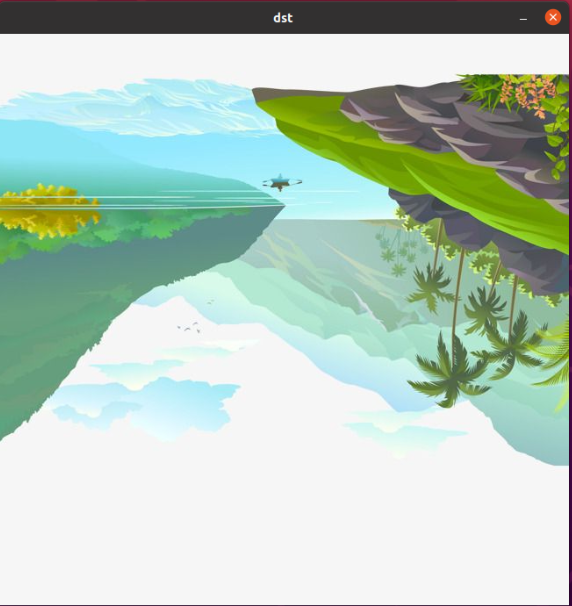
\includegraphics[width=0.5\linewidth]{rotate.png}
    \captionof{Rotação a 180º graus}
    \label{fig:rotate}
    \end{figure}
    
    \paragraph{}
   	\textbf{Executar programa:} ../opencv-example-bin/ex\textunderscore 2 <input\textunderscore file> r
   	
   	\begin{figure}[h!]
    \centering
    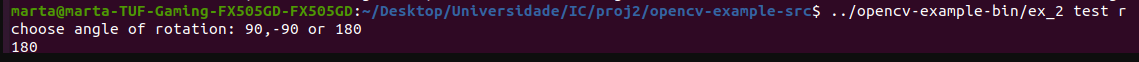
\includegraphics[width=1\linewidth]{formadecompilarrotacao.png}
    \captionof{Exemplo de compilação para criar versão rotacionada}
    \label{fig:compile}
    \end{figure}
    \paragraph{}
    \paragraph{}
   	\item \textbf{Aumentar ou diminuir intensidade de luz da imagem.}
    \paragraph{}
    Nesta implementação, usamos a função \textit{convertTo} do \textit{OpenCV}. Neste caso, os parâmetros de entrada da função são: o ficheiro de imagem destino onde irá ser guardado o resultado do efeito, -1 dado que o número de canais da matriz de imagem destino vai ser igual à origem, 1 pois não queremos alterações na escala, e \textit{value} que pode ser um valor negativo ou positivo.\paragraph{} Este \textit{value} vai ser adicionado a cada píxel. Se este for negativo vai haver uma diminuição de brilho, caso contrário vai existir um aumento.
   	\begin{scriptsize}
    \estiloC
   	\begin{lstlisting}[caption={Código fonte em C++ para aumentar ou diminuir a intensidade de luz da imagem}, label=lst:javacode]
    if(effect=="l"){ //https://www.opencv-srf.com/2018/02/change-brightness-of-images-and-videos.html
        cout<<"To increase light insert a positive <value> to decrease insert a negative <value>\n";
        int value;
        cout<<"choose value: "<<endl;
        cin>>value;
        Mat imageBrighnessHigh;
        if(value>0){
            image.convertTo(imageBrighnessHigh, -1, 1, value); //increase the brightness
            imshow("light_increase",imageBrighnessHigh);
            waitKey(0);
        }
        
        Mat imageBrighnessLow;
        if (value<0){
            image.convertTo(imageBrighnessLow, -1, 1, value); //decrease the brightness
            imshow("light_decrease",imageBrighnessLow);
            waitKey(0);
        }
    
        
        return 0;
    }
    \end{lstlisting}    
    \end{scriptsize}
   	
   	\begin{figure} [h!]
    \centering
    \begin{minipage}{.5\textwidth}
    \centering
    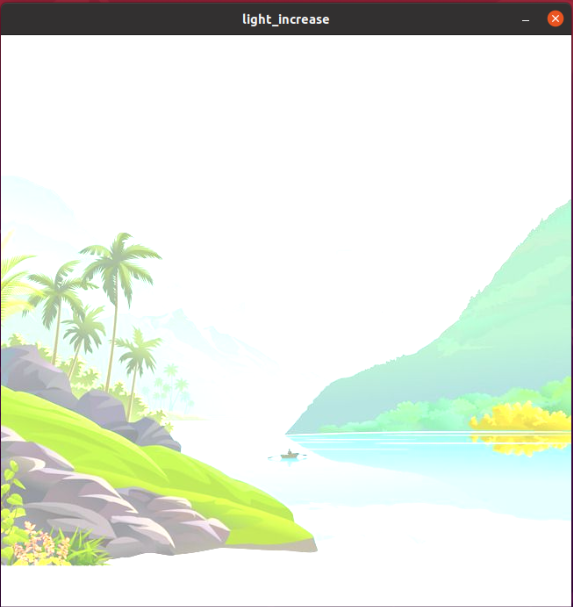
\includegraphics[width=0.8\linewidth]{light_increase.png}
    \captionof{Aumento da Intensidade}
    \label{fig:light_increase}
    \end{minipage}%
    \begin{minipage}{.5\textwidth}
    \centering
    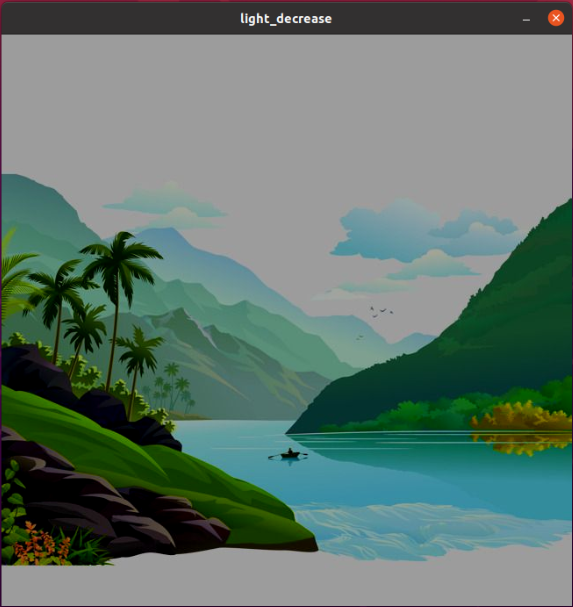
\includegraphics[width=.8\linewidth]{light_decrease.png}
    \captionof{Diminuição da Intensidade}
    \label{fig:light_decrease}
    \end{minipage}
    \end{figure}
    
    \paragraph{}
    \begin{figure}[h!]
    \centering
    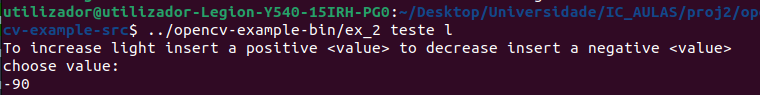
\includegraphics[width=1\linewidth]{formadecompilar_f.png}
    \captionof{Exemplo de compilação da diminuição da intensidade}
    \label{fig:compile}
    \end{figure}

    \end{enumerate}
 
\chapter{Parte II}
\label{chap.ParteII}
\section{Exercício 3}
\paragraph{}
Neste exercício, foi nos pedido para implementar uma classe para uma codificação de \textit{Golomb}. Esta permite gerar um conjunto de códigos de tamanho variável livres de prefixo que podem ser utilizados na compressão de dados. \paragraph{}
O código Golomb é uma família de códigos que dependem de um parâmetro inteiro, m > 0 onde,

\begin{equation}
    m = \left\lceil\dfrac{-1}{log \alpha}\right\rceil
\end{equation}
\paragraph{}

A codificação envolve separar um inteiro em duas partes: a parte unária e a parte binária. 
Dado que queremos codificar um número inteiro, n, este é representado por 2 números, q e r: \paragraph{}
\begin{equation}
    q = \left\lfloor\dfrac{n}{m}\right\rfloor
\end{equation}
\begin{equation}
    r = n - qm  
\end{equation}

\paragraph{}
O quoeficiente \textit{q} pode ter valores 0, 1, 2, 3... e dessa forma é representado pelo seu código unário correspondente.
\paragraph{}
O resto da divisão, \textit{r}, pode assumir valores entre 0 e m-1 e irá representar o respetivo código binário.
\paragraph{}
Esta situação, descrita anteriormente, é válida para quando o valor de m é uma potência de 2. Se não o for, o processo anteriormente descrito não é valido, sendo o método alternativo apresentado de seguida.\paragraph{}

\begin{itemize}
    \item Começamos por definir um valor b que nos diz quantos bits serão necessários para a parte binária da codificação Golomb.
    \begin{equation}
    b = \lceil log_2m \rceil
    \end{equation}
    \item Se \(r < 2^b- m\), o valor de de r é codificado em binário usando b-1 bits.
    \item Caso contrário, é codificado o valor \(r + 2^b -m\) em binário com b bits.
\end{itemize}


	\begin{scriptsize}
    \estiloC
   	\begin{lstlisting}[caption={Código fonte em C++ Classe Golomb: Codificar}, label=lst:javacode]
int Golomb::encode(int n){
    n = fold(n);
    int q = floor((int)(n / m));
    int r = n - (q * m);

    int nbitsbin;  // stores the number os bits of the binary part
    int value;     // value to be coded in the binary part

    // Verify if m is a power of two
    if ((m & (m-1)) == 0 && m != 0) {
        nbitsbin = b;
        value = r;
    }
    else{
        int x = pow(2, b) - m;
        // Verify if r is smaller than x
        if (r < x){  
            nbitsbin = b - 1;
            value = r;
        }
        else{
            nbitsbin = b;
            value = r + x;
        }
    }

    \end{lstlisting}    
    \end{scriptsize}

\paragraph{}

Um dos atributos desta classe vai ser um objeto da classe Bitstream, desenvolvida no projeto anterior, a qual é utilizada para escrever as codificações ou então lê-las no caso da descodificação. 

\paragraph{}
O processo da descodificação envolve ler bits escritos num ficheiro. Começa-se por contar o número de 0's (do código unário). Tendo o número de 0's descobrimos o valor da parte unária (U) que será depois multiplicado por m.
De seguida o processo terá duas alternativas dependendo se o valor de m for ou não uma potência de 2.

Caso seja, serão lidos \textit{b} bits que corresponderão ao valor de R, sendo o valor descodificado obtido através da soma de R com o da parte unária multiplicada por m (mU + R).

Caso o valor de m não seja uma potência de 2, serão lidos \textit{b - 1} bits e dependendo do valor lido haverão duas possibilidades para o cálculo do valor descodificado. Se este valor for inferior a x, tendo em conta que x=\((2^b - m)\), R será igual a este valor e o valor descodificado será obtido da mesma forma que foi descrita na situação anterior (mU + R).

Por outro lado se o valor lido for superior a x, será lido mais um bit, sendo o valor de R atualizado com este valor e o valor descodificado será dado pela expressão anterior subtraída pelo valor de x ((mU + R) - x).

\paragraph{}

	\begin{scriptsize}
    \estiloC
   	\begin{lstlisting}[caption={Código fonte em C++ Classe Golomb: Descodificar}, label=lst:javacode]
int Golomb::decode(){
    int U = 0;  // number of bits of the unary part
    int R = 0;  // number of bits of the rest
    int bit;    // current bit

    while(true){
        bit = file.readBit();
        if(bit == 1) break;
        U++;
    }
    // cout << "U= " << U << endl;
    // Verify if m is a power of two
    if ((m & (m-1)) == 0 && m != 0) {
        // vector<int> bin = file.readNbits(b); //reads the binary part
        int aux = b-1;
        for(int i = b-1; i >= 0; i--){
            bit = file.readBit();
            // cout << bit<< endl; 
            if (bit != 0){
                R += pow(2, aux);
            }
            aux--;
        }
        // cout << "R= " << R << endl;
        return unfold(m*U + R);
    }
    else {
        vector<int> bin = file.readNbits(b-1); //read b-1 bits from the binary part
        // cout << "b= " << b << endl;
        int aux = b-2;
        
        for(int i = 0; i < b-1; i++){
            if (bin[i] != 0){
                R += pow(2, aux);
            }
            aux--;
        }

        int x = (pow(2, b) - m);
        if(R < x){        
            // cout << "R= " << R << endl;
            return unfold(m*U + R); 
        }
        else{
            R = 2 * R; // "shift" of the bits that have been read 
            int Lsbit = file.readBit();
            if (Lsbit == 1){
                R++;
            }
            // cout << "x= " << x << endl;
            // cout << "R= " << R << endl;
            return unfold((m*U + R) - x); 
        }
    }
}



    \end{lstlisting}    
    \end{scriptsize}
    \paragraph{}
    
De forma a permitir a codificção de valores negativos, utilizamos um método em que os números negativos são representados por números ímpares positivos e
os números positivos são representados pelos pares. Esses métodos são representado pelas funções \textit{fold} e \textit{unfold} da classe \textit{Golomb}.
\paragraph{}

Para testar esta classe desenvolvemos o programa de teste test\textunderscore golomb.cpp, que codifica valores positivos e negativos e que de seguida procede à descodficação dos mesmos de forma a verificar se existiram erros em algum destes processos. 

Neste programa são também testadas funções auxiliares que foram desenvolvidas com vista a facilitar o processo de codificação de ficheiros de áudio e imagem.

\paragraph{}
Para além disso foi também desenvolvido o programa  test\textunderscore golomb2.cpp que testa a função auxiliar que irá servir para codificar e descodificar os headers dos ficheiros de aúdio. 

	
\chapter{Parte III}
\label{chap.ParteIII}
\section{Exercício 4}
\paragraph{}
\subsection*{Preditores}
\paragraph{}O preditor linear usado para o cálculo dos residuais é o que está descrito nas seguintes
equações:
\paragraph{}

\begin{equation}
\left\{
\begin{array}{c}
     \hat{X}_n^{(0)} = 0  \\
     \hat{X}_n^{(1)} = x_{n-1} \\
     \hat{X}_n^{(2)} = 2x_{n-1} - x_{n-2} \\
     \hat{X}_n^{(3)} = 3x_{n-1} - 3x_{n-2} + x_{n-3}
     
\end{array}
\right.    
\end{equation}



Após o cálculo especificado no seguinte sistema
de equações, faltava calcular o valor dos residuais que é dado por:
\begin{equation}
    r_n = x_n - \hat{x}_n
\end{equation}

Na reconstrução dos valores obtidos pelos preditores realiza-se a operação inversa:
\begin{equation}
    x_n = r_n - \hat{x}_n
\end{equation}

Logo, é necessário calcular \^{x}\textsubscript{n} que é dado pelos preditores que mencionámos anteriormente. No entanto, em vez de serem utilizados os valores originais das samples, vão ser usados os valores dos residuais obtidos.

\paragraph{}

Para conseguirmos obter uma entropia mais baixa, desenvolvemos o nosso código de forma a que o processamento de som seja feito canal a canal, isto é, o preditor está dividido em 2 uma parte para o canal esquerdo e outra para o canal direito. \paragraph{}
Portanto, o preditor faz as suas previsões para o canal esquerdo baseando-se na informação do canal esquerdo e faz as suas previsões no canal direito baseando-se na informação do canal direito. \paragraph{}
No entanto, os residuais resultantes desta previsão de cada canal são colocados no mesmo vetor.

\subsection*{Lossless Codec}

\paragraph{}Para testar este codec é necessário compilar e correr o ficheiro test\textunderscore audioCodec.cpp com um argumento de entrada que é o ficheiro a ser comprimido. Ao executar o ficheiro irá ser apresentado um prompt ao utilizador onde ele irá escolher o tipo de codec a usar. Neste caso, irá escolher a opção correspondente a lossless e de seguida o modo do preditor pretendido.
\paragraph{} 
Para a implementação deste codec é necessário recolher os dados referentes ao ficheiro de áudio que serão precisos para que a reconstrução do ficheiro original no lado do
descodificador seja possível. Logo, para esse efeito foi criada uma função adicional na classe Golomb que
permite a codificação do cabeçalho que vai conter informação crucial na reconstrução do ficheiro original. 

A informação contida num cabeçalho de áudio inclui o valor m que será utilizado pela classe Golomb, os campos associados ao ficheiro de áudio (nº de samples, sampleRate, formato e nº de canais), de seguida o modo do preditor utilizado, o modo do codificador (lossy ou lossless) e, por fim, o campo opcional que apenas existirá caso o codificador esteja em modo lossy que representa o número de bits a descartar no processo de quantização.

\begin{center}
\begin{tabular} { | p {3 cm} | p {3 cm}|p {3 cm}|p {3 cm}|p {3 cm}|}
    \hline
    Golomb m & 32 bits    \\
    \hline
    Número de Samples   & 32 bits \\
    \hline
    Sample Rate  & 32 bits \\
    \hline
    Format  & 32 bits \\
    \hline
    Channels  & 4 bits \\
    \hline
    PredMode  & 2 bits \\
    \hline
    Lossy  & 1 bits \\
    \hline
    shQuant & 5 bits \\
    \hline
    \end{tabular}
\end{center}
\paragraph{}
O valor de cada sample é enviado para o preditor que, por sua vez, irá calcular um valor que será utilizado para obter os residuais, r. Obtendo os residuais (r) calculamos o m ideal para codificar os residuais com códigos de Golomb. 
O método escolhido para calcular este valor é apresentado de seguida:
\begin{equation}
    mean = \dfrac{\sum fold(r_n)}{N}
\end{equation}
\begin{equation}
     m = \left\lceil\dfrac{-1}{log_2 \left( \dfrac{mean}{mean | 1.0} \right) }\right\rceil
\end{equation}

Após ser calculado o m, são criados os cabeçalhos e escritos no ficheiro. Para terminar o processo são escritos no ficheiro destino os valores dos residuais codificados através de códigos de
Golomb . Isto é feito através de  chamadas sucessivas à função \textit{encode} da classe Golomb.

\paragraph{}
Por sua vez, o processo descodificação é executado através das operações opostas às que foram descritas anteriormente. Este processo é iniciado ao ler primeiro o cabeçalho através da função desenvolvida na classe Golomb. Ao ler o cabeçalho obtemos o m e outros dados que nos permitem reconstruir o ficheiro original  \paragraph{} Tendo processado esta informação procedemos à leitura e descodificação de todos os valores dos residuais calculados. Essa leitura é feita com sucessivas chamadas à função decode da classe Golomb.
\paragraph{}
Para finalizar, após estes processos, vão ser copiados todos os dados obtidos no processamento de informação para um ficheiro àudio de output com recurso aos métodos da classe \textit{libsndfile}.

\section{Exercício 5}
\subsection*{Lossy Codec}
\paragraph{}Para testar este codec é necessário compilar e correr o mesmo ficheiro indicado anteriormente: test\textunderscore audioCodec.cpp com um argumento de entrada que é o ficheiro a ser comprimido. Aqui o utilizador irá escolher o codec lossy escolhendo de seguida o número de bits a serem descartados no processo de quantização e também o modo do preditor a utilizar.
\paragraph{}

Neste caso, a estrutura base é semelhante à descrita para o codec lossless.
A alteração efetuada foi a adição de um processo de quantização aos residuais calculados com o preditor.
E para isso foi também necessário alterar o preditor deste codec pois o cálculo dos residuais
tem de refletir esta quantização que é realizada. 
\paragraph{}
Assim sendo, sempre que é quantizado um residual, o valor usado nessa posição para o preditor é dado pelo soma de uma predição da
sample com o seu residual quantizado. 
\paragraph{}
A quantização é realizada com um shift à direita do número de bits indicado pelo utilizador.
Quando se atualiza o valor da sample para fazer o sincronismo do erro (soma da predição com
residual quantizado), é desfeito o shift (realizado na direção oposta o mesmo número de vezes).
\paragraph{}
O processo de descodificação é semelhante ao realizado no codec lossless. A diferença vai de encontro à necessidade de reconstruir a quantização que foi efetuada. Essa
reconstrução é feita efetuando um shift na direção oposta o mesmo número de vezes que foi realizada na codificação.

\subsection*{Resultados}
\paragraph{}Tendo em conta que,
\begin{equation}
    Compression \; ratio= \dfrac{Uncompressed \; File}{Compressed \; File}
\end{equation}

\begin{equation}
    Space \; saving = 1 - \dfrac{Uncompressed \; File}{Compressed \; File}
\end{equation}

apresentamos nas tabelas seguintes os resultados de vários testes efetuados aos codec de áudio. Desta forma iremos conseguir analisar e retirar conclusões sobre o desempenho e resultados obtidos dos codecs (primeiramente do codec lossless e de seguida do lossy). 
\paragraph{}
{\large \textbf{Lossless:}}
\paragraph{}
As colunas das tabelas representam, respetivamente, o modo do preditor utilizado, a taxa de compressão, o espaço salvo através da compressão do ficheiro e também a duração do processo de compressão.
\paragraph{}
\textbf{FILE: sample03.wav }
\begin{center}
%\paragraph{}
\begin{tabular} { | p {2 cm} | p {2 cm} | p {2.5 cm}| p {2 cm} | }
    \hline
    PredMode&CompRatio &SpaceSaving(\%) &Duration(s) \\
    \hline
    1& 1.466236& 31.798133&6.211558  \\
    \hline
    2& 1.525929& 34.466134 &5.995765 \\
    \hline
    3& 1.500377& 33.350083 & 6.418600 \\
    \hline
    \end{tabular}
\end{center}

\textbf{FILE: sample04.wav }
\begin{center}
%\paragraph{}
\begin{tabular} { | p {2 cm} | p {2 cm} | p {2.5 cm}| p {2 cm} | }
    \hline
    PredMode&CompRatio &SpaceSaving(\%) &Duration(s) \\
    \hline
    1& 1.366147 & 26.801439 & 4.516673  \\
    \hline
    2& 1.549826 & 35.476615 & 3.888854 \\
    \hline
    3& 1.617674 & 38.182829 & 3.590187 \\
    \hline
    \end{tabular}
\end{center}

\textbf{FILE: sample05.wav }
\begin{center}
%\paragraph{}
\begin{tabular} { | p {2 cm} | p {2 cm} | p {2.5 cm}| p {2 cm} | }
    \hline
    PredMode&CompRatio &SpaceSaving(\%) &Duration(s) \\
    \hline
    1& 1.549500 & 35.463032 & 5.826299  \\
    \hline
    2& 1.725942 & 42.060627 & 5.498499 \\
    \hline
    3& 1.747565 & 42.777514 & 5.627314 \\
    \hline
    \end{tabular}
\end{center}

\textbf{FILE: sample06.wav }
\begin{center}
%\paragraph{}
\begin{tabular} { | p {2 cm} | p {2 cm} | p {2.5 cm}| p {2 cm} | }
    \hline
    PredMode&CompRatio &SpaceSaving(\%) &Duration(s) \\
    \hline
    1& 1.778635 & 43.777119 & 5.836242  \\
    \hline
    2& 2.255081 & 55.655695 & 5.065854\\
    \hline
    3& 2.549906 & 60.782871 & 4.417672 \\
    \hline
    \end{tabular}
\end{center}
\paragraph{}
Analisando os resultados obtidos para os diferentes ficheiros de áudio, é possível concluir que em geral, o preditor 3 obteve os melhores resultados tanto a nível de taxa de compressão como a nível de duração do processo de compressão, o que significa que, para além de ter a capacidade de comprimir mais os ficheiros também o consegue fazer de forma mais eficiente.
\paragraph{}
{\large \textbf{Lossy} (PredMode = 2): }
\paragraph{}
Neste caso as colunas das tabelas representam, respetivamente, o número de bits a descartar no processo de quantização, a taxa de compressão, o espaço salvo através da compressão do ficheiro, a duração do processo de compressão e também o SNR (Signal-to-noise ratio) obtido ao comparar o ficheiro restaurado (após a compressão) com o seu original.
\paragraph{}
\textbf{FILE: sample03.wav }
\begin{center}
\begin{tabular} {  |p {2 cm} | p {2 cm} | p {2.5 cm}| p {2 cm} | p {2 cm} |}
    \hline
    BitsQuant&CompRatio &SpaceSaving(\%) &Duration(s) & SNR(dB)\\
     \hline
    1& 1.686861& 40.718293 &5.427951  & 71.9986\\
    \hline
    2& 1.885766 & 46.971161 &5.430606 & 63.5509\\
    \hline
    3& 2.137650 & 53.219667 & 4.718977 & 56.5616\\
    \hline
    4& 2.466756 & 59.460922 & 4.452133 & 50.1023\\
    \hline
    5& 2.911542& 65.653938 & 3.525287 & 43.863\\
     \hline
    7& 4.318189 & 76.842145 & 2.328813 & 31.6593\\
    \hline
    9& 6.557065 & 84.749275 & 1.518348 & 19.5806\\
     \hline
    11& 10.94079& 90.859892 & 0.839566 & 7.48592\\
     \hline
    13& 13.454509 & 92.567548 & 0.728113 & -4.91724\\
    \hline
    \end{tabular}
\end{center}
\paragraph{}
É possível concluir que conforme o número de bits que serão removidos no processo de quantização aumenta, a taxa de compressão, por sua vez, também aumenta, tal como seria esperado. Isto deve-se ao facto de serem considerados cada vez menos bits para representar cada amostra o que levará a uma poupança de espaço necessário para armazenar o ficheiro comprimido.
\paragraph{}
Conseguimos obervar que, quantos mais bits são removidos menor será o valor do SNR. Isto justifica-se pelo facto de que quando os bits são removidos são introduzidos erros na
fonte de informação e daí surge um aumento de ruído, que consequentemente levará a que o valor
do SNR diminua. Para o último valor do número de bits removidos, o ficheiro descomprimido apresenta quase só ruído.


\paragraph{}
{\large\textbf{Entropia (Lossy e lossless encoding, PredMode = 3)}}
\paragraph{}
Na tabela abaixo observamos a entropia associada ao ficheiro original e de seguida a obtida após o processo de predição dos codecs (lossless e lossy) para o caso do preditor 3, dado que, foi este que apresentou melhores resultados. 
\begin{center}
\begin{tabular} { | p {2 cm} | p {3 cm} | p {3 cm} | p {3 cm} |}
    \hline
    Audio File & Entropy (original) &Entropy (residuals, lossless) &Entropy (residuals, lossy)    \\
    \hline
    sample03.wav & 13.2678 & 10.441 & 8.46562 \\
    \hline
    sample04.wav & 14.1619 & 9.85233 & 7.85467 \\
    \hline
    sample05.wav & 12.4516 & 8.68766 & 6.83448 \\
    \hline
    sample06.wav & 11.8349 & 6.05798 & 4.16605 \\
    \hline
    \end{tabular}
\end{center}
\paragraph{}
Para ambos os codecs conseguimos concluir que o preditor atingiu o seu objetivo. 
A sua finalidade era obter uma sequência de valores cuja entropia fosse menor que a sequência de valores original, isto é, menos símbolos binários necessários para codificar a fonte de informação.

Por fim, conclui-se também que entropia associada aos residuais obtidos através do preditor do codec lossy foi ligeiramente menor que a do codec lossless. O facto de a entropia ser menor implica, consequentemente, uma maior taxa de compressão o que conseguimos verificar pelos resultados obtidos anteriormente.
\paragraph{}
Para executar o programa para os processos de codificação lossless e lossy:\paragraph{}
\textbf{Executar programa:} ../opencv-example-bin/test\textunderscore audiocodec <input file>
\paragraph{}
E de seguida, deve ser selecionado o modo do codificador pretendido (0 para lossless e 1 para lossy), posteriormente é selecionado o modo do preditor (1, 2 ou 3) e, por fim, caso o codificador esteja em modo lossy é também pedido ao utilizador que este insira o número de bits a descartar no processo de quantização (valor entre 1 e 15). 

\chapter{Parte IV}
\label{chap.ParteIV}
\section{Exercício 6}

\paragraph{}
\subsection*{Preditor}
\paragraph{}
O preditor usado para este codec foi não linear e as suas equações são descritas como indicamos a seguir:
\begin{equation}
\hat{x}=
\left\{
\begin{array}{c}
     min(a, b) \; if \; c \geq \; max(a, b)  \\
     max(a, b) \; if \; c \leq \; min(a, b)\\
     a + b - c \; otherwise
\end{array}
\right.  
\end{equation}

\paragraph{}

A base deste preditor é a mesma da configuração espacial do JPEG:
\begin{center}
    \begin{figure} [h!]
    \centering
    \centering
    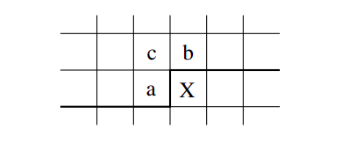
\includegraphics[width=1\linewidth]{conf_espacial.png}
    \captionof{Configuração espacial do JPEG}
    \label{fig:configuracao_espacial}
    \end{figure}
\end{center}
\subsection*{Lossless image}
\paragraph{}

A estrutura deste codec é baseada na estrutura que foi descrita no exercício 4.
Por isso, o preditor utilizado já foi descrito na secção anterior. A diferença deste codec para o de aúdio está no processamento.
\paragraph{}
A transformação rgb <-> YCbCr usada foi 8-bit full-range é descrita na imagem abaixo:

\begin{center}
    \begin{figure} [h!]
    \centering
    \centering
    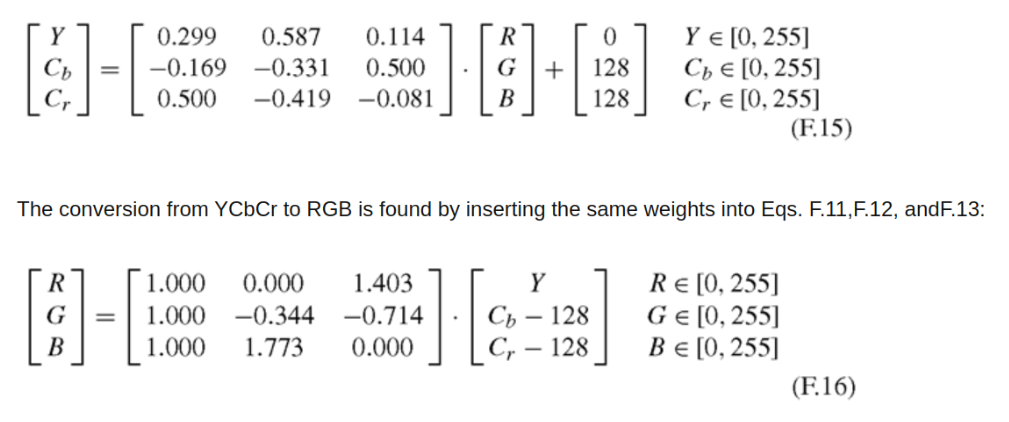
\includegraphics[width=1\linewidth]{conversion.png}
    \captionof{Fórmulas usadas para conversão RGB <-> YCbCr}
    \label{fig:conversão_RGB_YCbCr}
    \end{figure}
\end{center}

De seguida, é preciso manipular o tamanho das componentes Cr e Cb, porque estas necessitam serem \textit{sub-sampling} do tipo 4:2:0. \paragraph{}
As componentes Cb e Cr são 1/4 do tamanho em área em relação à imagem principal, logo no resize RGB -> YCbCr é feita a
média entre 4 valores adjacentes da mesma componente e é esse valor que representa essa componente no novo tamanho.
\paragraph{}
Resumidamente, cada bloco de entrada é convertido do espaço de cores RGB para o espaço de cores YCbCr. A transformação usada usa um valor de entrada RGB com cada componente no intervalo [0 - 255] e transforma-o em Y, Cb e Cr, nos intervalos [0, 0, 255, 0], [-128, 0, 127, 0] e [-128, 0, 127, 0], respetivamente. O componente Y é deslocado para baixo em 128, de modo que também caia na faixa [-128, 0, 127, 0]. 
\paragraph{}
Para o cálculo do m do Golomb, usámos a média ponderada dos residuais após a operação \textit{fold} em vez da média aritmética pois foram obtidos melhores resultados com este tipo de média. Todo o restante processo de cálculo foi semelhante ao utilizado para os ficheiros de áudio.

\subsection*{Resultados}
\paragraph{}
\begin{center}
    \begin{figure} [h!]
    \centering
    \centering
    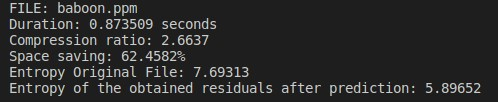
\includegraphics[width=1\linewidth]{baboonEncode.jpeg}
    \captionof{Baboon Encode}
    \label{fig:baboon_encode}
    \end{figure}
\end{center}

\begin{center}
    \begin{figure} [h!]
    \centering
    \centering
    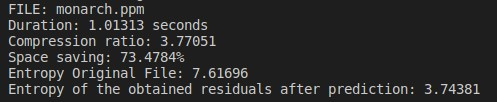
\includegraphics[width=1\linewidth]{monarchEncode.jpeg}
    \captionof{Monarch Encode}
    \label{fig:monarch_encode}
    \end{figure}
\end{center}

	\begin{figure} [h!]
    \centering
    \begin{minipage}{.6\textwidth}
    \centering
    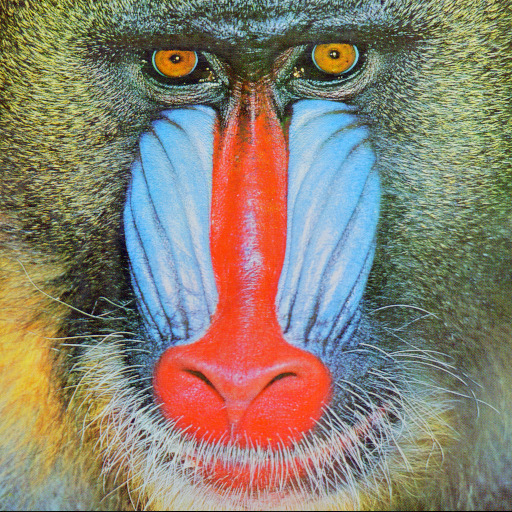
\includegraphics[width=0.9\linewidth]{baboon.jpg}
    \captionof{Baboon original image}
    \label{fig:light_increase}
    \end{minipage}%
    \begin{minipage}{.6\textwidth}
    \centering
    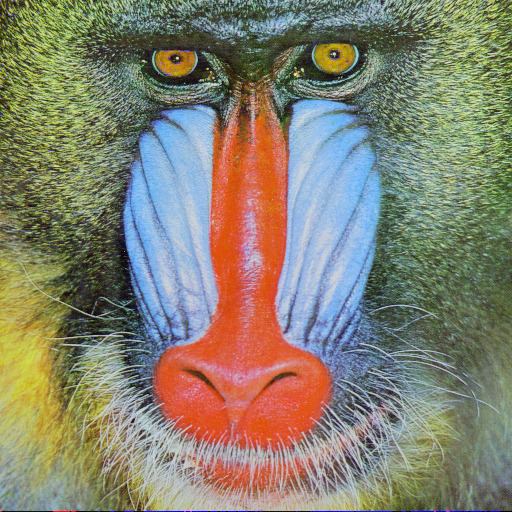
\includegraphics[width=0.9\linewidth]{restoredbaboon.jpg}
    \captionof{Restored\textunderscore image}
    \label{fig:light_decrease}
    \end{minipage}
    \end{figure}
    
    

	\begin{figure} [h!]
    \centering
    \begin{minipage}{.6\textwidth}
    \centering
    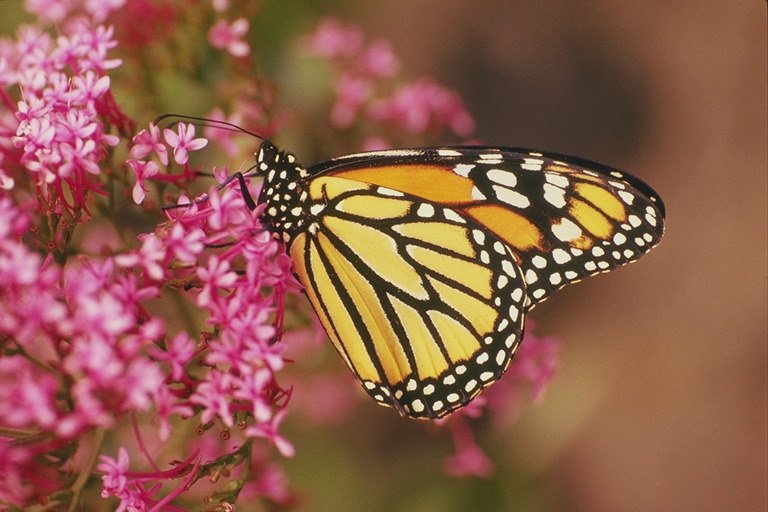
\includegraphics[width=0.9\linewidth]{monarch.jpg}
    \captionof{monarch original image}
    \label{fig:light_increase}
    \end{minipage}%
    \begin{minipage}{.6\textwidth}
    \centering
    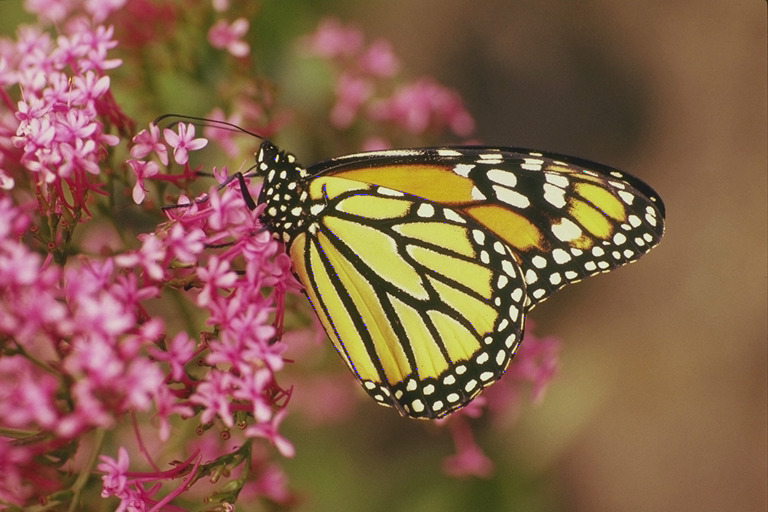
\includegraphics[width=0.9\linewidth]{restoredmonarch.jpg}
    \captionof{Restored\textunderscore image}
    \label{fig:light_decrease}
    \end{minipage}
    \end{figure}
\newpage
Observamos que quanto menor a entropia calculada nos residuais a serem
codificados, maior é a taxa de compressão do ficheiro.
\paragraph{}

\textbf{Executar Programa}../opencv-example-bin/test\textunderscore imageCodec <inputfile>

\chapter*{Contribuições dos autores}
\paragraph{}
O trabalho foi dividido entre os três, sendo as percentagens para cada um as seguintes:
\paragraph{}
Bruno Silva -> 35\%
\paragraph{}
Marta Oliveira -> 35\%
\paragraph{}
Mariana Silva -> 30\%

\chapter*{Webgrafia}

%%%%%%%%%%%%%%%%%%%%%%%%%%%%%%%%%
\paragraph{}
\url{https://elearning.ua.pt/pluginfile.php/3743066/mod_resource/content/4/ic-notas.pdf}
\paragraph{}
\url{https://stackoverflow.com/questions/14907964/mirror-image-in-opencv}
\paragraph{}
\url{https://www.opencv-srf.com/2018/02/change-brightness-of-images-and-videos.html}
\paragraph{}
\url{https://stackoverflow.com/questions/32190494/what-is-the-vec3b-type}

%\printbibliography

\end{document}
